\section{Design und Implementierung einer Schnittstelle für maschinelles Lernen}\label{sec:aiInterface}

Wie im Einführungskapitel beschrieben ist es ein Ziel des Projektes, eine Grundlage für ein weiteres Projekt mit dem Thema \textit{maschinelles Lernen} (engl. \textit{machine learning}) zu schaffen. Dazu wird eine Schnittstelle benötigt, über die mithilfe der im vorherigen Kapitel beschriebenen Serialisierung und Deserialisierung Informationen über den Spielstand übertragen und Teile des Spiels gesteuert werden können.

\subsection{Umfang der Schnittstelle}\label{sec:interfaceDesign}

Die Schnittstelle umfasst eine Steuerung und Ausgabe relevanter Informationen für die Nicht-Spieler-Charaktere, mit dem Ziel, eine Verbesserung der Benutzererfahrung durch maschinelles Lernen zu ermöglichen. Dabei wäre es beispielsweise denkbar, dass sich die Schwierigkeit der Gegner an die Spielweise des Nutzers anpasst.

Gesteuert werden die Bewegungen der Charaktere inklusive Blickrichtung und Geschwindigkeit, die Attacken mit und ohne Waffe sowie die Interaktionen mit Gegenständen in der Umgebung. Außerdem ermöglicht die Schnittstelle einen Abbruch der Steuerung, die bewirkt, dass der Gegner zu seinem Standardverhalten zurückkehrt (siehe \ref{sec:enemyDesign}).

Zu den relevanten Informationen, die übergeben werden, gehören Informationen über den gesteuerten Charakter. Diese umfassen die am Prefab eingestellten Werte für den Charaktertyp, zum Beispiel die maximale Geschwindigkeit oder die Größe des Sichtfeldets, sowie charakterspezifische Eigenschaften wie die Waffe und die Menge an Munition. Ebenso wichtig sind Informationen über den Status des Charakters, darunter die verbleibende Anzahl an Leben sowie die aktuelle Position und Geschwindigkeit. Außerdem werden Informationen über das Level benötigt, insbesondere über die Objekte in der Umgebung sowie durch den Spieler verursachte Geräusche. Die Informationen über den Aufbau des Levels und die Spieler-Position werden dabei bewusst auf die direkte Umgebung des Charakters eingeschränkt, um die Entwicklung eines allwissenden Gegners zu verhindern.

\subsection{Vernetzung}\label{sec:interfaceSocket}

Eine Möglichkeit für die Erzeugung einer Schnittstelle zu einem anderen Programm ist der Unity-eigene Networkmanager \textit{UNet} \cite{Unity_Doc_UNet}, mit dem sehr leicht Verbindungen zu anderen Programmen hergestellt werden können. \textit{UNet} ist sehr mächtig, allerdings wird die Unterstützung in absehbarer Zeit eingestellt werden, da ein neues System entwickelt wird. Zudem wurde \textit{UNet} explizit für die Entwicklung von Multiplayer-Spielen entwickelt, weshalb der potenzielle Nutzer der Schnittstelle für seine Applikation ebenfalls an Unity gebunden wäre.

Da eine flexible, platformunabhängigen Schnittstelle erstrebenswert ist, sind \textit{TCP Sockets} die bessere Wahl \cite{Microsoft_Socket}. Dazu wird zu der Hauptszene des Spiels ein Controller hinzugefügt, der für die Schnittstelle zuständig ist. Dieser Controller hat eine Komponente namens \texttt{Socket-\linebreak Component}, die für die Herstellung der Verbindung sowie die Datenübertragung zuständig ist. Empfangene Daten werden für die Weiterverarbeitung an die ebenfalls am Controller hängende AIInterfaceComponent weitergegeben (siehe \ref{sec:interfaceControls}). Außerdem werden in einem festen Zeitabstand die Umgebungsdaten der aktiven Gegner an alle Clients übertragen (siehe \ref{sec:interfaceSerialization}).

Am Controller kann im Unity-Editor über die öffentlichen Variablen der Socket-Komponente der Zeitintervall für die Übertragung der Daten eingestellt werden sowie ob und an welchem Port eine Verbindung hergestellt werden soll.

\subsection{Steuerung eines Charakters}\label{sec:interfaceControls}

Um einen Charakter zu steuern, muss über die TCP-Verbindung ein Befehl im JSON-Format an das Unity-Spiel gesendet werden. Die Befehlsstruktur ist in der Klasse \texttt{JsonEnemyCommand- \linebreak Structure} definiert. Der Befehl enthält die ID des zu steuernden Charakters und den Namen des auszuführenden Befehls sowie gegebenenfalls notwendige Zusatzinformationen.

Empfangene Befehle werden durch die Socket-Komponente an die \texttt{AIInterface}-Komponente weitergeleitet, wo sie deserialisiert werden. Mithilfe des \texttt{PersonControllers} wird anhand der ID der richtige Gegner ermittelt und die entsprechende Methode der Schnittstellenkomponente des Gegners ausgeführt. Das Standardverhalten des Gegners wird daraufhin abgebrochen und es werden nur noch die Befehle ausgeführt, die von dem Socket empfangen werden.

Die Schnittstellenkomponente des Gegners hat folgende Methoden:

\begin{itemize}
	\item \texttt{SetDestination(Vector2 destination, float velocity)}
	\item \texttt{SetRotation(float rotation)}
	\item \texttt{FireWeapon()}
	\item \texttt{DropWeapon()}
	\item \texttt{CloseCombatAttack()}
	\item \texttt{StopOverride()}
	\item \texttt{Interact(string id)}
\end{itemize}

Mit der Methode \texttt{SetDestination(...)} kann ein neues Ziel festgelegt werden. Als Parameter werden die Zielkoordinaten sowie die Geschwindigkeit, mit der sich der Charakter bewegen soll, übergeben. Das Pfadfindung wird dabei von dem \texttt{NavAgent} des Charakters übernommen (siehe \ref{sec:pathfinding}). Über die Methode \texttt{SetRotation(...)} kann außerdem die Blickrichtung geändert werden.

Für die Attacken können die Methoden \texttt{FireWeapon()} und \texttt{CloseCombatAttack()} verwendet werden, mit \texttt{Interact(...)} und \texttt{DropWeapon()} können Waffen aufgenommen und abgelegt werden. Mit \texttt{StopOverride()} kann außerdem die externe Kontrolle des Gegners abgebrochen werden. Der Gegner kehrt daraufhin zu seinem Standardverhalten zurück.

Die IDs der aktiven Gegner sowie der interaktiven Objekte werden beim Start des Spiels generiert und können den Umgebungsdaten entnommen werden. Die ausführbaren Befehle heißen so wie die Methoden der Schnittstellenkomponente des Gegners. Ein Befehl könnte also beispielsweise so aussehen:

\texttt{
\string{
\string"EnemyID": "16a04a3a-57e2-453a-a132-3bc1543153a2",
"Method": \newline\string"SetDestination",
"Destination": \string{
"x": 12,
"y": 14
\string},
"Velocity": 3
\string}
}

\subsection{Serialisierung der Umgebungsdaten}\label{sec:interfaceSerialization}

Wie bereits beschrieben werden die für die aktiven Gegner relevanten Informationen regelmäßig über das Socket versendet. Um sicherzustellen, dass die Schnittstelle genau die Daten übergibt, die für den Gegner relevant sind, ohne dass dieser allwissend sein kann, müssen die Attribute des Gegners sowie alle Objekte im Sichtfeld des Gegners (siehe Kapitel \ref{sec:enemyImplementationAwareness}) serialisiert werden. 

Das bedeutet jedoch, dass der bestehende Level-Serializer (siehe \ref{sec:designSerialization}) hier nicht verwendet werden kann, da dieser explizit zum Serialisieren ganzer Levels entwickelt wurde. Hinzu kommt, dass hier Objekte serialisiert werden müssen, die zum Speichern des Levels nicht benötigt werden und dass bei den zu serialisierenden Objekten andere Attribute relevant sind. Außerdem kann zwischen den Objekten im Sichtfeld des Gegners und den Data-Objekten des Level-Controllers keine Verbindung hergestellt werden, sodass diese für die Serialisierung nicht verwendet werden können.

Deshalb werden eine eigene Klasse für die Serialisierung der für die Schnittstelle relevanten Daten und eigene Strukturen für die Serialisierten Objekte entwickelt.

In einem nächsten Schritt könnten die Serialisierungssysteme für das Level und für die Umgebungsdaten konsolidiert werden. Dies könnte beispielsweise mithilfe von \textit{Reflection} umgesetzt werden (siehe \cite{Reflection}).

\subsection{Implementierung einer Webapplikation}\label{sec:interfaceExample}

Zur Demonstration der Schnittstelle wird eine kleine Webapplikation geschrieben. Das Backend ist in \textit{NodeJS} geschrieben und stellt eine Verbindung zum TCP-Socket des Unity-Spiels her. Das Frontend ist mit \textit{VueJS} umgesetzt und wird im Sekundentakt aktualisiert. Die Verbindung zwischen Frontend und Backend ist mit \textit{axios} implementiert, das \textit{Routing} funktioniert mit \textit{Express}.

Im Frontend werden zur besseren Übersicht nicht alle Daten ausgegeben, sondern nur, wie in Abbildung \ref{fig:webapp} zu sehen ist, der Gegnertyp, die verbleibenden Leben, der Waffentyp und die Menge an Munition sowie die aktuelle Position und Blickrichtung. Für die verfügbaren Aktionen gibt es Schaltflächen.

\begin{figure}[h]
 \centering
 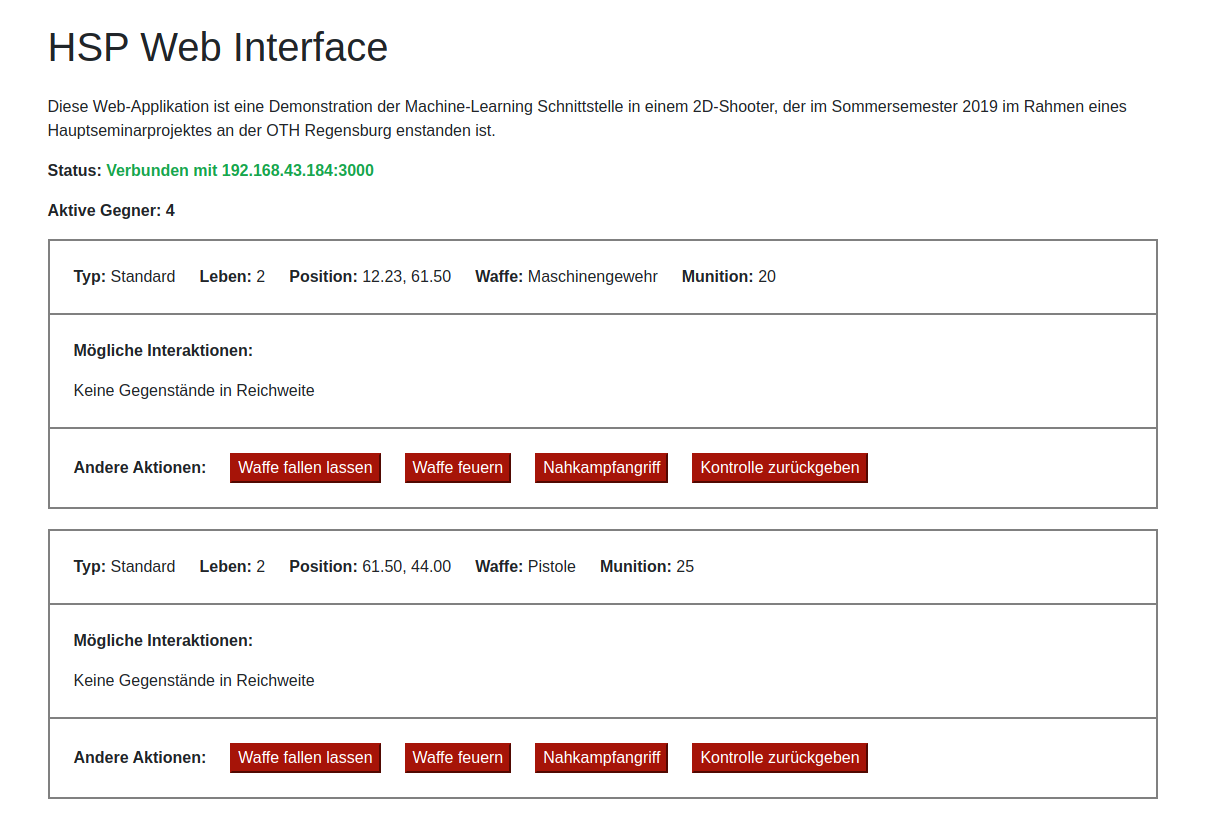
\includegraphics[width=0.835\linewidth]{pics/web-app_connected.png}
 \captionof{figure}[Demo-Applikation]{Benutzeroberfläche der Demo-Applikation}
	\label{fig:webapp}
\end{figure}

Die Applikation demonstriert nicht nur die Funktionsfähigkeit der Schnittstelle, sondern auch, dass die Programmiersprache bei der Entwicklung einer künstlichen Intelligenz zur Steuerung der Gegner keine Rolle spielt.

\subsection{Möglichkeiten der Schnittstelle}\label{sec:interfacePossibilities}

Die Schnittstelle bietet nicht nur eine Grundlage für die Forschung mit maschinellem Lernen, sondern könnte leicht erweitert werden. Es würde sich beispielsweise anbieten, die \texttt{Person} Hierarchie und die Schnittstelle so anzupassen, dass nicht nur Gegner gesteuert werden können, sondern auch der Spieler. Dies könnte auch für eine Analyse von Spielerverhalten interessant sein.

In jedem Fall sollte die Fehlerbehandlung der Schnittstelle verbessert werden, insbesondere der Umgang mit falschem Input sowie mit Verbindungsproblemen. Außerdem wäre es sinnvoll, die Optionen für die Verbindung in das Hauptmenü aufzunehmen.
